Let, given vector
 \begin{equation}
  \vec{P} = \myvec{3 \\ 8}
 \end{equation}
%Let, given vector $\vec{P} = \myvec{3 \\ 8}\\ $

    
Let, image point be $\vec{R} $. 
Let vector,
\begin{equation}
 \vec{n}  = \myvec{1 \\ 3}
\end{equation}
Let m be the directional vector along the line,  
\myvec{1 & 3} $\vec{x}$ =7   
Hence m is,
\begin{equation}
\vec{m} = \myvec{3 \\ -1} 
\end{equation}
 


\begin{figure}[!ht]
\centering

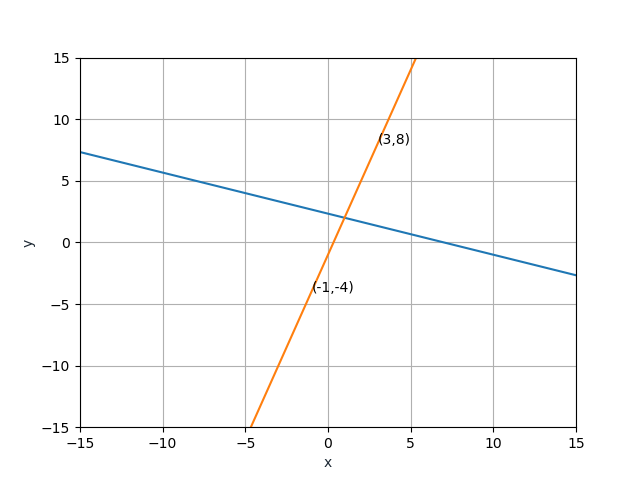
\includegraphics[width=\columnwidth]{./solutions/line_plane/55/Figure_1.png}
\caption{Image of a point in 2D line}
\label{fig1:solutions/line_plane/55/}
\end{figure}
By property in Figure \ref{fig1:solutions/line_plane/55/}, the line PR bisects the mirror equation perpendicularly. Hence, 
\begin{equation}
    2\vec{Q} = \vec{P} + \vec{R}
\end{equation}
Where, $\vec{Q}$ is the point on the line,  \myvec{1 & 3} $\vec{x}$ =7.
Hence the reflection vector $\vec{R}$ is given as, 
\begin{equation}
    \brak{ \frac{\vec{R}}{2}} = \brak{\frac{\vec{m}\vec{m}^T - \vec{n}\vec{n}^T}{\vec{m}^T\vec{m} + \vec{n}^T  \vec{n}}}\vec{P} + c \brak{\frac{\vec{n}}{\norm{\vec{n}}^2}}    \label{eq::solutions/line_plane/55/2}
\end{equation}



\begin{align}
     \norm{\vec{n}} = \sqrt{1^2+3^2} = \sqrt{10}
\end{align}
   
 

  
 
 
Substituting these values in equation \eqref{eq::solutions/line_plane/55/2} we get,
\begin{equation}
\vec{R} = \myvec{-1 \\ -4} 
\end{equation}
Hence, it is the required answer for image of $\vec{P}$ in line \myvec{1 & 3} $\vec{x}$ =7. 
 
 

 

